\documentclass[11pt]{article}

\usepackage[letterpaper, margin=2.5cm]{geometry}
\usepackage{amsmath}
\usepackage{amssymb}
\usepackage{amsthm}
\usepackage{graphicx}
\usepackage{caption}
\usepackage{subcaption}
\usepackage{multirow}
\usepackage{placeins}

\graphicspath{{images/}}

\let\bld\boldsymbol
\newtheorem{theorem}{Theorem}

\bibliographystyle{plain}

\title{Discontinuous Galerkin method with Taylor basis functions}
\author{Aditya Kashi}
\date{April 24, 2017}

\begin{document}

\maketitle
\begin{abstract}
Discontinuous Galerkin (DG) finite element method (FEM) with Taylor basis theoretically has several advantages over traditional nodal Lagrange basis FEM for the numerical solution of hyperbolic problems. We wish to investigate theoretically and numerically a Taylor basis DG FEM. One of the advantages of using Taylor basis functions is that reconstructing higher order derivatives becomes straightforward, which is the key idea in the `reconstructed' DG (RDG) method. We would like to investigate the effectiveness of this method as well.
\end{abstract}

\section{Introduction}
We wish to investigate the solution of hyperbolic problems in two-dimensions using Taylor basis functions in a discontinuous Galerkin (DG)) finite element method (FEM). Nodal Lagrange finite elements are by far the most commonly used as the polynomial basis of choice in fields like solid mechanics and fluid mechanics. However, an alternative exists in modal basis functions, such as Legendre basis and Taylor basis.

There are some advantages that the hierarchical, modal, Taylor basis functions have over nodal Lagrange basis functions \cite{luo_taylor, aizinger_scaleseparation}. 
\begin{itemize}
\item The set of basis functions of a certain polynomial degree contains the basis functions of all lower-degree sets of basis functions, ie., the basis is \emph{hierarchical}. This makes easier the implementation of p-adaptation (dynamically changing polynomial degree locally based on accuracy requirements during the simulation) and p-multigrid solvers (utilizing corrections to the solution computed from lower-order solves).
\item The Taylor basis expansion remains same and the basis functions retain the same form irrespective of the geometric type of elements. This makes for easier implementation of codes that work both on triangles and quadrangles, or all three of tetrahedra, prims and hexahedra. Another aspect of this is that the number of degrees of freedom in case of Taylor basis is smaller than that in case of nodal basis for non-simplicial elements, while maintaining optimal order of accuracy.
\item Thirdly, they make implementation of reconstruction DG methods (described later) efficient and elegant. This is because the spatial derivatives of the unknowns are readily available as those are the degrees of freedom. Using them, higher derivatives can be reconstructed to improve the accuracy of the scheme, as done in high-order (higher than 1st order) finite volume methods.
\end{itemize}

\section{Governing equations}

A hyperbolic partial differential equation in $n_d$ spatial dimensions can be written as
\begin{equation}
\frac{\partial \bld{u}}{\partial t} + \sum_{j=1}^{n_d} \frac{\partial \bld{F}_j}{\partial x_j} = \bld{0} \quad \bld{x} \in \Omega, t \in [0,T]
\label{conservativeGE}
\end{equation}
with some initial condition
\begin{equation}
\bld{u}(\bld{x},0) = \bld{u}_0(\bld{x})
\end{equation}
and some combination of several possible types of boundary conditions.
$\bld{u}(\bld{x},t) \in \mathbb{R}^m$ is the vector of the $m$ conserved variables and $\bld{F}_j(\bld{u}(\bld{x},t)) \in \mathbb{R}^m$ are the flux functions. For a compact notation, we define a flux `matrix' $\bld{F}$ as the matrix with the x- and y- fluxes as the columns. We can then write \eqref{conservativeGE} as
\begin{equation}
\bld{u}_t + \nabla\cdot\bld{F}(\bld{u}) = \bld{0}
\label{conservativetensorGE}
\end{equation}
where $\nabla\cdot$ is now the tensor divergence and $\bld{F} \in \mathbb{R}^{m\times n_d}$. This means $\bld{F}:\mathbb{R}^{n_d}\rightarrow \mathbb{R}^m$ maps any vector (direction) in space to the flux in that direction. Note that the operator $\bld{F}$ is a function of the state $\bld{u}$.

Here, we consider the steady 2-dimensional linear advection equation.
\begin{equation}
\nabla\cdot(\bld{\beta}u) = f, \quad \bld{x} \in [-\frac32,\frac32]\times[-1,1]
\end{equation}
where $f(x,y) = \frac{2\pi}{3}\cos\frac{2\pi}{3}(x+\frac32)$, $\bld{\beta} = (1,0)$ and the true solution $u(x,y) = \sin\frac{2\pi}{3}(x+\frac32)$. We solved it here by iterating in `pseudo-time' to steady state using explicit time-stepping.
\begin{equation}
\frac{\partial u}{\partial \tau} + \nabla\cdot(\bld{\beta}u) = f
\end{equation}

\section{Finite element formulation}

A weak formulation is derived in a `broken' Sobolev space and discretized by finite element method \cite{luo_taylor}. For $w \in W$, a suitable test function space, we can multiply \eqref{conservativetensorGE} by $w$ and integrate over an element $\Omega_e$. Taking $\mu$ as the domain measure and $s$ as the boundary measure,
\begin{equation}
\int_{\Omega} \frac{\partial u}{\partial t}w\,d\mu + \int_{\Omega}\nabla\cdot\bld{F}(u)w \,d\mu = \bld{0}.
\end{equation}
However, we cannot necessarily integrate by parts to obtain a weak form because the function space $W$ is not necessarily regular enough. We thus derive a discrete weak form on each element as described below.

Let $\mathcal{T}_h$ be a set of subsets of $\Omega_h$ such that $\bigcup_{K\in \mathcal{T}_h}K = \Omega_h$ and $K_i \cap K_j = \phi \, \forall K_i, K_j \in \mathcal{T}_h, i \neq j$, and $\partial K$ is a Lipschitz boundary for all $K \in \mathcal{T}_h$. Our choice of the discrete function space is, for some positive integer $k$,
\begin{align}
W_{K} &:= P_k(K), \quad K \in \mathcal{T}_h \\
W_h &:= \bigoplus_{K \in \mathcal{T}_h} W_{K}
\end{align}
where $P_k(K)$ is the space of $k$th degree polynomials on set $K$ and $\bigoplus$ denotes a direct sum \cite{nodaldg}.

We can then state the discrete weak formulation on each element as follows. Find $u_h \in W_{K}$ such that
\begin{equation}
\int_{K} \frac{\partial u_h}{\partial t}w\,d\mu + \int_{\partial K} \bld{F}(u_h)\cdot\hat{\bld{n}}w \,ds - \int_{K}\bld{F}(u_h)\cdot\nabla w \,d\mu = \bld{0} \quad \forall w \in W_{K},\, K \in \mathcal{T}_h.
\label{wf}
\end{equation}
In the above weak form, note that $\hat{\bld{n}}$ is the unit outward normal to $\partial K$.

Consider basis $b_i(\bld{x})$ on an element $K$ of the mesh $\mathcal{T}_h$. We can then write $u_h = \sum_{j=1}^n u_j b_j(\bld{x})$. Further, we introduce the numerical flux $h$ defined such that for a face $f$ between two elements $\Omega_L$ and $\Omega_R$ with states (conserved variables) $\bld{u}_L$ and $ \bld{u}_R$,
\begin{equation}
\bld{F}(u)\cdot\hat{\bld{n}}_f \approx h(\bld{u}_L, \bld{u}_R, \hat{\bld{n}}_f).
\end{equation}
This is necessary because $u$ is, in general, discontinuous across element interfaces $f$ and the analytical flux $\bld{F}(u)\hat{\bld{n}}_f$ is not uniquely defined.

The discrete form becomes: find the $n$ degrees of freedom (DOFs) $u_j$ of each conserved variable $\mathbf{u} \in \mathbb{R}^n$, such that (note: $\bld{u}_L, \bld{u}_R$ still denote functions in the discrete space $W_{K}^m$)
\begin{equation}
\sum_{j=1}^n\int_{K} b_ib_j\,d\mu\, \frac{d\mathbf{u}}{d t} + \int_{\partial K}  h(\bld{u}_L(\bld{x}), \bld{u}_R(\bld{x}), \hat{\bld{n}})b_i \,ds - \int_{K}\bld{F}(u_h(\bld{x}))\cdot\nabla b_i \,d\mu = \bld{0}, \quad i \in {1,...n},\, K \in \mathcal{T}_h.
\label{df}
\end{equation}

We thus need to solve the following ODE on each element.
\begin{equation}
M \frac{d\mathbf{u}}{dt} + \bld{r}(\mathbf{u}(t)) = \bld{0}
\label{ode}
\end{equation}
where $M \in \mathbb{R}^{n\times n}$ is the mass matrix $[M]_{ij} = \int_{K} B_iB_j\,d\mu$ and $\bld{r}(\mathbf{u})$ is the vector: $\bld{r}_i(\mathbf{u}) :=  \int_{\partial K}  \bld{h}(\bld{u}_{hL}, \bld{u}_{hR}, \hat{\bld{n}})b_i \,ds - \int_{\Omega_e}\bld{F}(u_h)\nabla b_i \,d\mu$. Note that we have given the equation for one conserved variable, and that the coupling between the different conserved variables comes about from the flux $\bld{F}$ and numerical flux $h$.

In our implementation, Gauss-Legendre quadrature has been used to integrate the terms in the weak form. The number of points was chosen so that a polynomial of degree 2$p$ would be integrated exactly for $p$th degree basis functions.

\section{Taylor basis functions}
In a Taylor basis, a function is expressed as a Taylor expansion about the element center. In 2D, a quadratic or P2 expansion in an element e would be written as
\begin{equation}
u_h = u_c + \frac{\partial u}{\partial x} \Big|_c(x-x_c) + \frac{\partial u}{\partial y} \Big|_c(y-y_c) + \frac{\partial^2 u}{\partial x^2} \Big|_c \frac{(x-x_c)^2}{2} + \frac{\partial^2 u}{\partial y^2} \Big|_c \frac{(y-y_c)^2}{2} + \frac{\partial^2 u}{\partial x\partial y} \Big|_c (x-x_c)(y-y_c)
\label{eqn:taylorexpn_orig}
\end{equation}
where the subscript `c' indicates the quantity at the element's geometric center. Let $A_e$ be the element area. Then we can take an average of both sides over the element to get
\begin{multline}
\tilde{u} = u_c + \frac{\partial u}{\partial x} \Big|_c \frac{1}{A_e}\int_{\Omega_e}(x-x_c)d\mu + \frac{\partial u}{\partial y} \Big|_c \frac{1}{A_e}\int_{\Omega_e} (y-y_c)d\mu \\ \, + \frac{\partial^2 u}{\partial x^2} \Big|_c \frac{1}{A_e}\int_{\Omega_e} \frac{(x-x_c)^2}{2}d\mu + \frac{\partial^2 u}{\partial y^2} \Big|_c \frac{1}{A_e}\int_{\Omega_e} \frac{(y-y_c)^2}{2}d\mu + \frac{\partial^2 u}{\partial x\partial y} \Big|_c \frac{1}{A_e}\int_{\Omega_e} (x-x_c)(y-y_c)d\mu \\
= u_c + \frac{\partial^2 u}{\partial x^2} \Big|_c \frac{1}{A_e}\int_{\Omega_e} \frac{(x-x_c)^2}{2}d\mu + \frac{\partial^2 u}{\partial y^2} \Big|_c \frac{1}{A_e}\int_{\Omega_e} \frac{(y-y_c)^2}{2}d\mu + \frac{\partial^2 u}{\partial x\partial y} \Big|_c \frac{1}{A_e}\int_{\Omega_e} (x-x_c)(y-y_c)d\mu
\end{multline}
where $\tilde{u}$ is the average value of the unknown function over the element, and $\mu$ is the area measure in 2D. This last equation can be subtracted from \eqref{eqn:taylorexpn_orig} to get
\begin{multline}
u_h = \tilde{u} + \frac{\partial u}{\partial x} \Big|_c(x-x_c) + \frac{\partial u}{\partial y} \Big|_c(y-y_c) + \frac{\partial^2 u}{\partial x^2} \Big|_c \left( \frac{(x-x_c)^2}{2} - \frac{1}{A_e}\int_{\Omega_e} \frac{(x-x_c)^2}{2}d\mu \right) \\ + \frac{\partial^2 u}{\partial y^2} \Big|_c \left( \frac{(y-y_c)^2}{2} -\frac{1}{A_e}\int_{\Omega_e} \frac{(y-y_c)^2}{2}d\mu \right) + \frac{\partial^2 u}{\partial x\partial y} \Big|_c \left( (x-x_x)(y-y_x) - \frac{1}{A_e}\int_{\Omega_e} (x-x_x)(y-y_x)d\mu \right).
\label{eqn:taylorexpn}
\end{multline}
This gives us our basis functions and corresponding degrees of freedom on a physical element $\Omega_e = K$. We also normalize the basis functions to get a better-conditioned discrete problem. Finally, the basis functions used for a P2 `Taylor finite element' are
\begin{align}
&B_1(\bld{x}) = 1 
\label{eq:taylorbasis0} \\
&B_2(\bld{x}) = \frac{(x-x_c)}{\Delta x} \\
&B_3(\bld{x}) = \frac{(y-y_c)}{\Delta y} \\
&B_4(\bld{x}) = \left( \frac{(x-x_c)^2}{2\Delta x^2} - \frac{1}{|K|}\int_{K} \frac{(x-x_c)^2}{2}d\mu \right) \\
&B_5(\bld{x}) = \left( \frac{(y-y_c)^2}{2\Delta y^2} -\frac{1}{|K|}\int_{K} \frac{(y-y_c)^2}{2}d\mu \right) \\
&B_6(\bld{x}) = \left( \frac{(x-x_c)(y-y_c)}{\Delta x\Delta y} - \frac{1}{|K|}\int_{K} (x-x_c)(y-y_c)d\mu \right)
\label{eq:taylorbasis}
\end{align}
($|K|$ is the measure of element $K$) with the corresponding coefficients, the degrees of freedom, being
\begin{align}
\tilde{U} := \tilde{u} \\
U_x := \frac{\partial u}{\partial x}\Big|_c \Delta x \\
U_y := \frac{\partial u}{\partial y}\Big|_c \Delta y \\
U_{xx} := \frac{\partial^2 u}{\partial x^2}\Big|_c \Delta x^2 \\
U_{yy} := \frac{\partial^2 u}{\partial y^2}\Big|_c \Delta y^2 \\
U_{xy} := \frac{\partial^2 u}{\partial x\partial y}\Big|_c \Delta x\Delta y
\label{eq:taylordofs}
\end{align}
where $\Delta x$ and $\Delta y$ are $\frac12 (x_{max}-x_{min})$ and $\frac12 (y_{max}-y_{min})$ respectively, and subscripts max and min indicate maximum and minimum values over the element. Note that symbols such as $U_x$ include their respective normalization factors.

\subsection{The Taylor basis finite element}
As defined by Ciarlet, a finite element is a triplet $(K, P_K, \Sigma_K)$ where $K$ is a compact connected Lipschitz subset of $\mathbb{R}^n$ with nonempty interior, $P_K$ is a finite dimensional vector space of functions $K \rightarrow \mathbb{R}^p$, $p \in \mathbb{N}$ and $\Sigma_K$ is a finite set of linear functionals $P_K \rightarrow \mathbb{R}$ called the local degrees of freedom. For a valid finite element, the set of local degrees of freedom must be \emph{unisolvent}, ie., the functionals in $\Sigma_K$ must be linearly independent and the cardinality of $\Sigma_K$ must equal the dimension of $P_K$.

That the Taylor basis functions can be used to define a finite element in the sense of Ciarlet can be shown as follows.
\begin{theorem}
The Taylor element defined by \eqref{eq:taylorbasis0} - \eqref{eq:taylordofs} on an element $K$ is unisolvent.
\end{theorem}
\begin{proof} We define $P_K$ and $\Sigma_K$ on a mesh element $K$ as follows.
\begin{multline}
P_K = \mathbb{P}_2(K), \\
L_1(u) := \frac{1}{|K|}\int_K u d\mu,\, L_2(u) := \frac{\partial u}{\partial x}\Big|_c \Delta x,\, L_3(u) := \frac{\partial u}{\partial y}\Big|_c \Delta y \\
L_4(u) := \frac{\partial^2 u}{\partial x^2}\Big|_c 2\Delta x^2,\,
L_5(u) := \frac{\partial^2 u}{\partial x\partial y}\Big|_c \Delta x\Delta y,\,
L_6(u) := \frac{\partial^2 u}{\partial y^2}\Big|_c 2\Delta y^2, \quad u \in P_K,\\
\Sigma_K = \{L_1, L_2, ... L_6\}
\end{multline}
where c represents the value at the center of the element, ie., at $\bld{r}_c = 1/|K|\int_K \bld{r}d\mu$. Clearly, the number of functionals in $\Sigma_K$ is equal to the dimension of $\mathbb{P}_2(K)$, and each functional is clearly linear because of the linearity of integrals and partial derivatives. Now suppose $\sum_{i=1}^6 c_i L_i = 0$, ie.,
\begin{equation}
\sum_{i=1}^6 c_i L_i(f) = 0 \quad \forall f \in P_K.
\end{equation}
Setting $f = c$, a constant, we see that $c_1$ has to be zero. If we set $f = ax+b$ with $\int_K f d\mu = 0$, we get $c_2$ = 0. We find that $f(x,y) := x-x_c$. Similarly, from $f(x,y) = y-y_c$, we obtain $c_3 = 0$.

Next, we choose $f = ax^2+bx+c$ such that $\int_K f d\mu = 0$, that is, \[f(x,y) = (x-x_c)^2 - 1/|K|\int_K(x-x_c)^2d\mu, \] we get $c_4 = 0$. Similarly, choosing $f(x,y) = (x-x_c)(y-y_c) - 1/|K|\int_K(x-x_c)(y-y_c)d\mu$ and $f(x,y) = (y-y_c)^2 - 1/|K|\int_K(y-y_c)^2d\mu$, we obtain $c_5 = 0$ and $c_6 = 0$. Thus the functionals in $\Sigma_K$ are linearly independent, and the element is unisolvent. This can be similarly extended to any desired polynomial degree in any number of dimensions.
\end{proof}

It has been shown by Johnson and Pitk\"aranta \cite{johnson_pitkaranta} that the following error estimate holds for $\mathbb{P}_k$ finite elements for scalar linear hyperbolic equations on shape-regular and quasi-uniform meshes:
\begin{equation}
\lVert u-u_h \rVert_{L^2(\Omega)} \leq h^{k+1/2} |u|_{H^{k+1}(\Omega)}.
\end{equation}
Since we have proved that the Taylor element is a valid finite element, the same proof holds for Taylor elements as well. Note that in practice, we generally achieve $O(h^{k+1})$ convergence, though there are some rare cases which make the above estimate sharp.

An interesting point is that the Taylor basis functions above are defined on the physical element. Thus, any polynomial function of these functions or their gradients remains polynomial. This means that terms in the mass matrix and stiffness matrix (for polynomial flux functions) can be integrated exactly by Gaussian quadrature of high-enough order, \emph{even for curved elements}. This may be contrasted to how Lagrange basis functions are defined on physical elements (see, for example, chapter 12 in \cite{claesjohnson}). The finite-dimensional function space on element $K$ is defined as
\begin{equation}
P_K = \{ p: p(\bld{x}) = \hat{p}(F^{-1}(\bld{x})),\, \bld{x} \in K,\, \hat{p} \in P_{\hat{K}} \}
\end{equation}
where $F:\hat{K}\rightarrow K$ is a diffeomorphism from the reference element $\hat{K}$ to the physical element $K$. For curved elements, $F^{-1}$ is not a polynomial in general. Thus, integrands in a weak form will, in general, not be polynomials and thus cannot be integrated exactly.

One disadvantage of Taylor basis is that since it is defined on physical elements, values of the basis functions and basis gradients at the quadrature points have to be stored individually for each element. This is not required in case of basis functions defined over the reference element.

\section{Reconstruction DG scheme}
An issue with the DG FEM method is its high cost compared to finite volume schemes for low to intermediate levels of desired accuracy. They become competitive only when a high-enough level of accuracy is required. DG FEM is also more expensive than a continuous FEM scheme of the same order on the same grid, since degrees of freedom are not shared among elements. One way of reducing the cost is the reconstruction DG (RDG) FEM scheme \cite{luo_rdg}. A Taylor basis RDG scheme can be implemented in a reasonably straightforward manner to give high-order accuracy using less degrees of freedom than a DG scheme. The main idea is that in regions where the solution is smooth enough, data from neighboring elements can be used to `reconstruct' a higher-order solution. However, as currently used, this is a reconstruction in the strong sense. This means that strong derivatives of the exact solution must exist if higher-order accuracy is to be attained.

Consider a DG P1 scheme with Taylor elements. The degrees of freedom are the mean value over the element and the first spatial derivatives at the element centre. Using this data, the three second spatial derivatives can be reconstructed using data from face-neighbouring elements, assuming a smooth enough solution in the region. Consider the union of a given element $\Omega_i$ and its face-neighbouring elements $\Omega_j$. In 2D, $j = 1,2,3$ or $j = 1,2,3,4$ when $\Omega_i$ is a triangle or quadrangle respectively. We write the unknown $u(x)$ as a Taylor series on this union (using the nomenclature introduced in the previous section).
\begin{equation}
u(\bld{x}) = \tilde{U}_i + U_{xi}B_{i_2}(\bld{x}) + U_{yi}B_{i_3}(\bld{x}) + U_{xxi} B_{i_4}(\bld{x}) + U_{yyi} B_{i_5}(\bld{x}) + U_{xyi} B_{i_6}(\bld{x})
\end{equation}
where $B$ are the basis functions on element $i$ and the derivatives are those at the centre of element $i$.

Note that we already know the first-order derivatives as those are our degrees of freedom. The second derivatives are the unknowns we wish to reconstruct. To this end, the above equation and its derivatives can be evaluated at the element-centres $\bld{x}_j$ of each of the face-neighbouring elements $j$.
\begin{align}
u_j &= \tilde{U}_i + U_{xi}B_{i_2}(\bld{x}_j) + U_{yi}B_{i_3}(\bld{x}_j) + U_{xxi} B_{i_4}(\bld{x}_j) + U_{yyi} B_{i_5}(\bld{x}_j) + U_{xyi} B_{i_6}(\bld{x}_j) \\
\frac{\partial u}{\partial x}\Big|_j &= U_{xi}/\Delta x_i + U_{xxi} B_{i_2}(\bld{x}_j) / \Delta x_i + U_{xyi} B_{i_3}(\bld{x}_j) /\Delta x_i \\
\frac{\partial u}{\partial y}\Big|_j &= U_{yi}/\Delta y_i + U_{xyi} B_{i_2}(\bld{x}_j) / \Delta y_i + U_{yyi}B_{i_3}(\bld{x}_j)/\Delta y_i
\end{align}
This can be expressed as the following linear system.
\begin{equation}
\begin{bmatrix}
B_4^j & B_5^j & B_6^j \\
B_2^j & B_3^j & 0 \\
0 & B_2^j & B_3^j
\end{bmatrix}
\begin{bmatrix}
U_{xxi} \\ U_{xyi} \\ U_{yyi}
\end{bmatrix} =
\begin{bmatrix}
u_j - (\tilde{U}_i + U_{xi}B_2^j + U_{yi}B_3^j) \\
\frac{\Delta x_i}{\Delta x_j}U_{xj} - U_{xi} \\
\frac{\Delta y_i}{\Delta y_j}U_{yj} - U_{yi}
\end{bmatrix} =:
\begin{bmatrix}
R_1^j \\ R_2^j \\ R_3^j
\end{bmatrix}
\end{equation}
where the superscript $j$ indicates that the function is evaluated at the element-centre of $j$. Writing these equations for all face-neighbours $j$, we get a 9x3 system for a triangle and a 12x3 system for a quadrilateral, in the three variables - the three second derivatives at the centre of cell $i$. This can be solved in a least squares sense to give a unique solution. Further, a WENO reconstruction can be used to suppress spurious oscillations to preserve nonlinear stability \cite{luo_hweno}.

\section{DG vs SUPG}
The `streamline upwind Petrov-Galerkin' method is a technique for solving hyperbolic PDEs that uses continuous trial and test function spaces, as opposed to DG methods. This means that degrees of freedom are shared between surrounding elements, and thus the number of degrees of freedom required to attain a given error level is lower than DG, at least for smooth solutions. SUPG is stable in presence shocks as well. However, it has its issues, as described nicely in section 2.5 of \cite{hartmann_thesis}.

\section{Results}

We present results for the forced linear advection equation described in section 2, using Taylor basis DG FEM for 1st and 2nd degree polynomial basis. We achieve optimal orders of accuracy on quadrilateral meshes as well, even though we use less degrees of freedom than a Lagrange DGFEM would use.

\begin{figure}
	\centering
	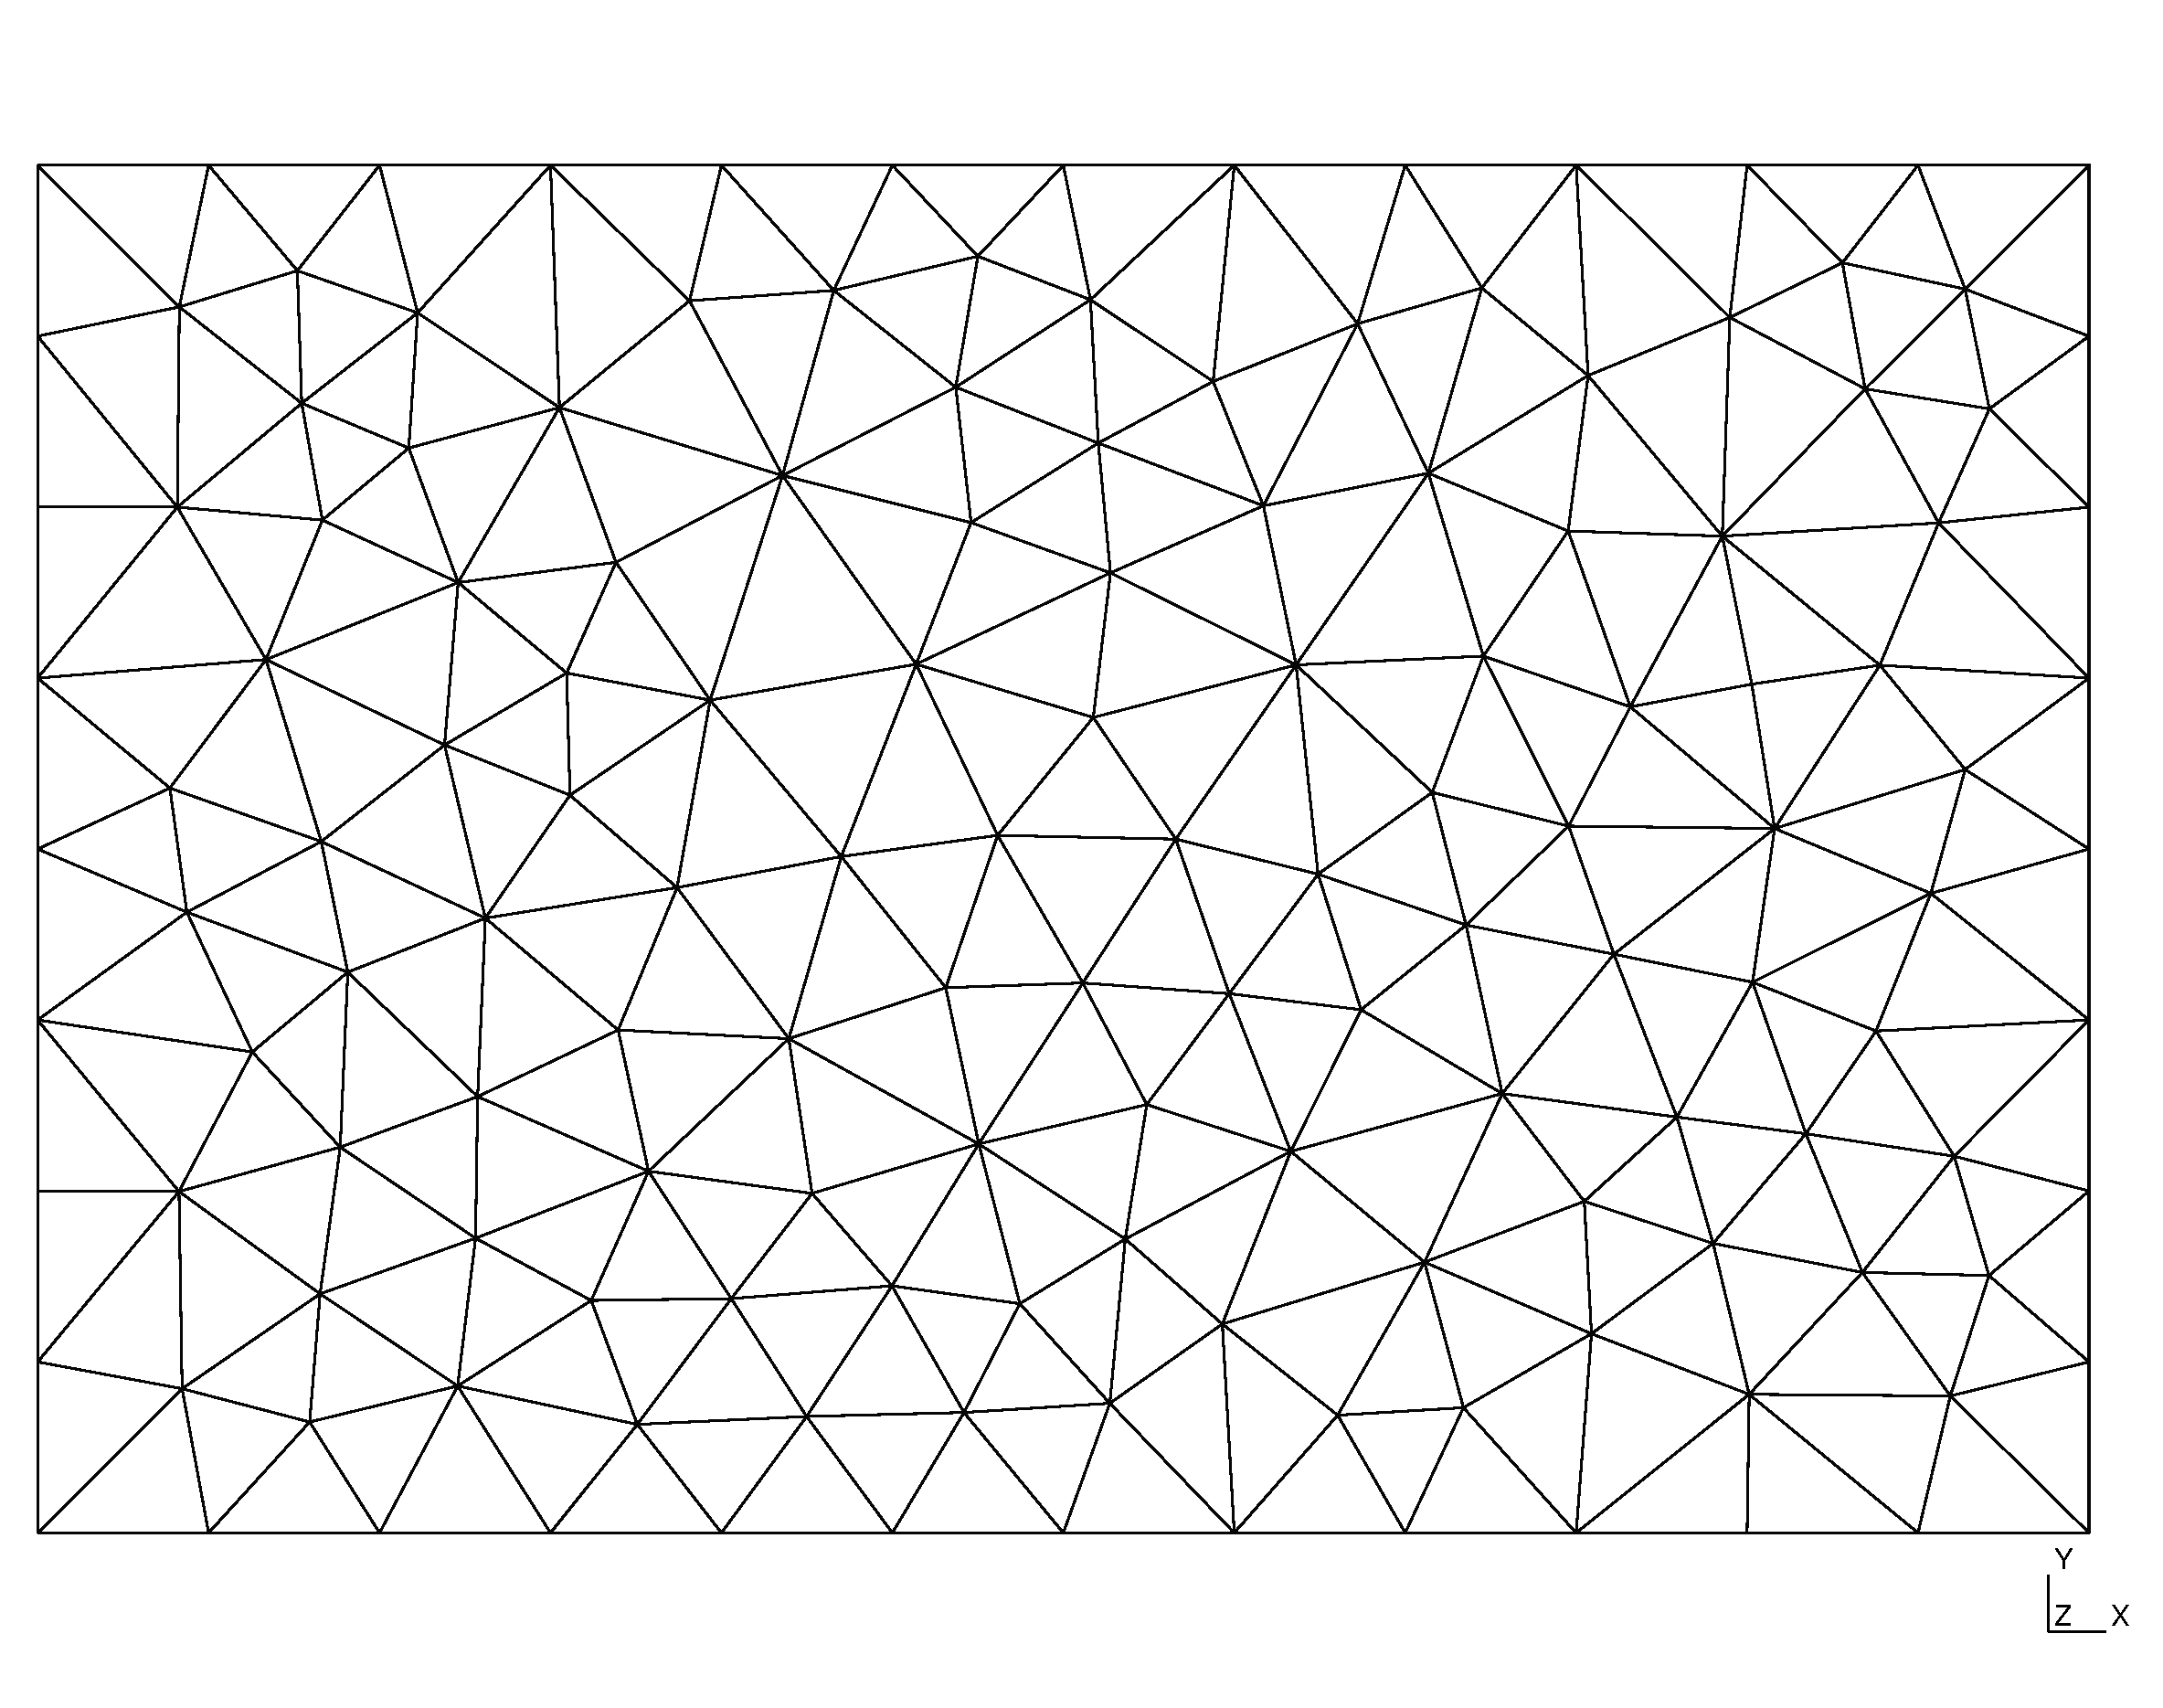
\includegraphics[scale=0.25]{meshtri}
	\caption{One of the triangular meshes used}
\end{figure}
\begin{figure}
	\centering
	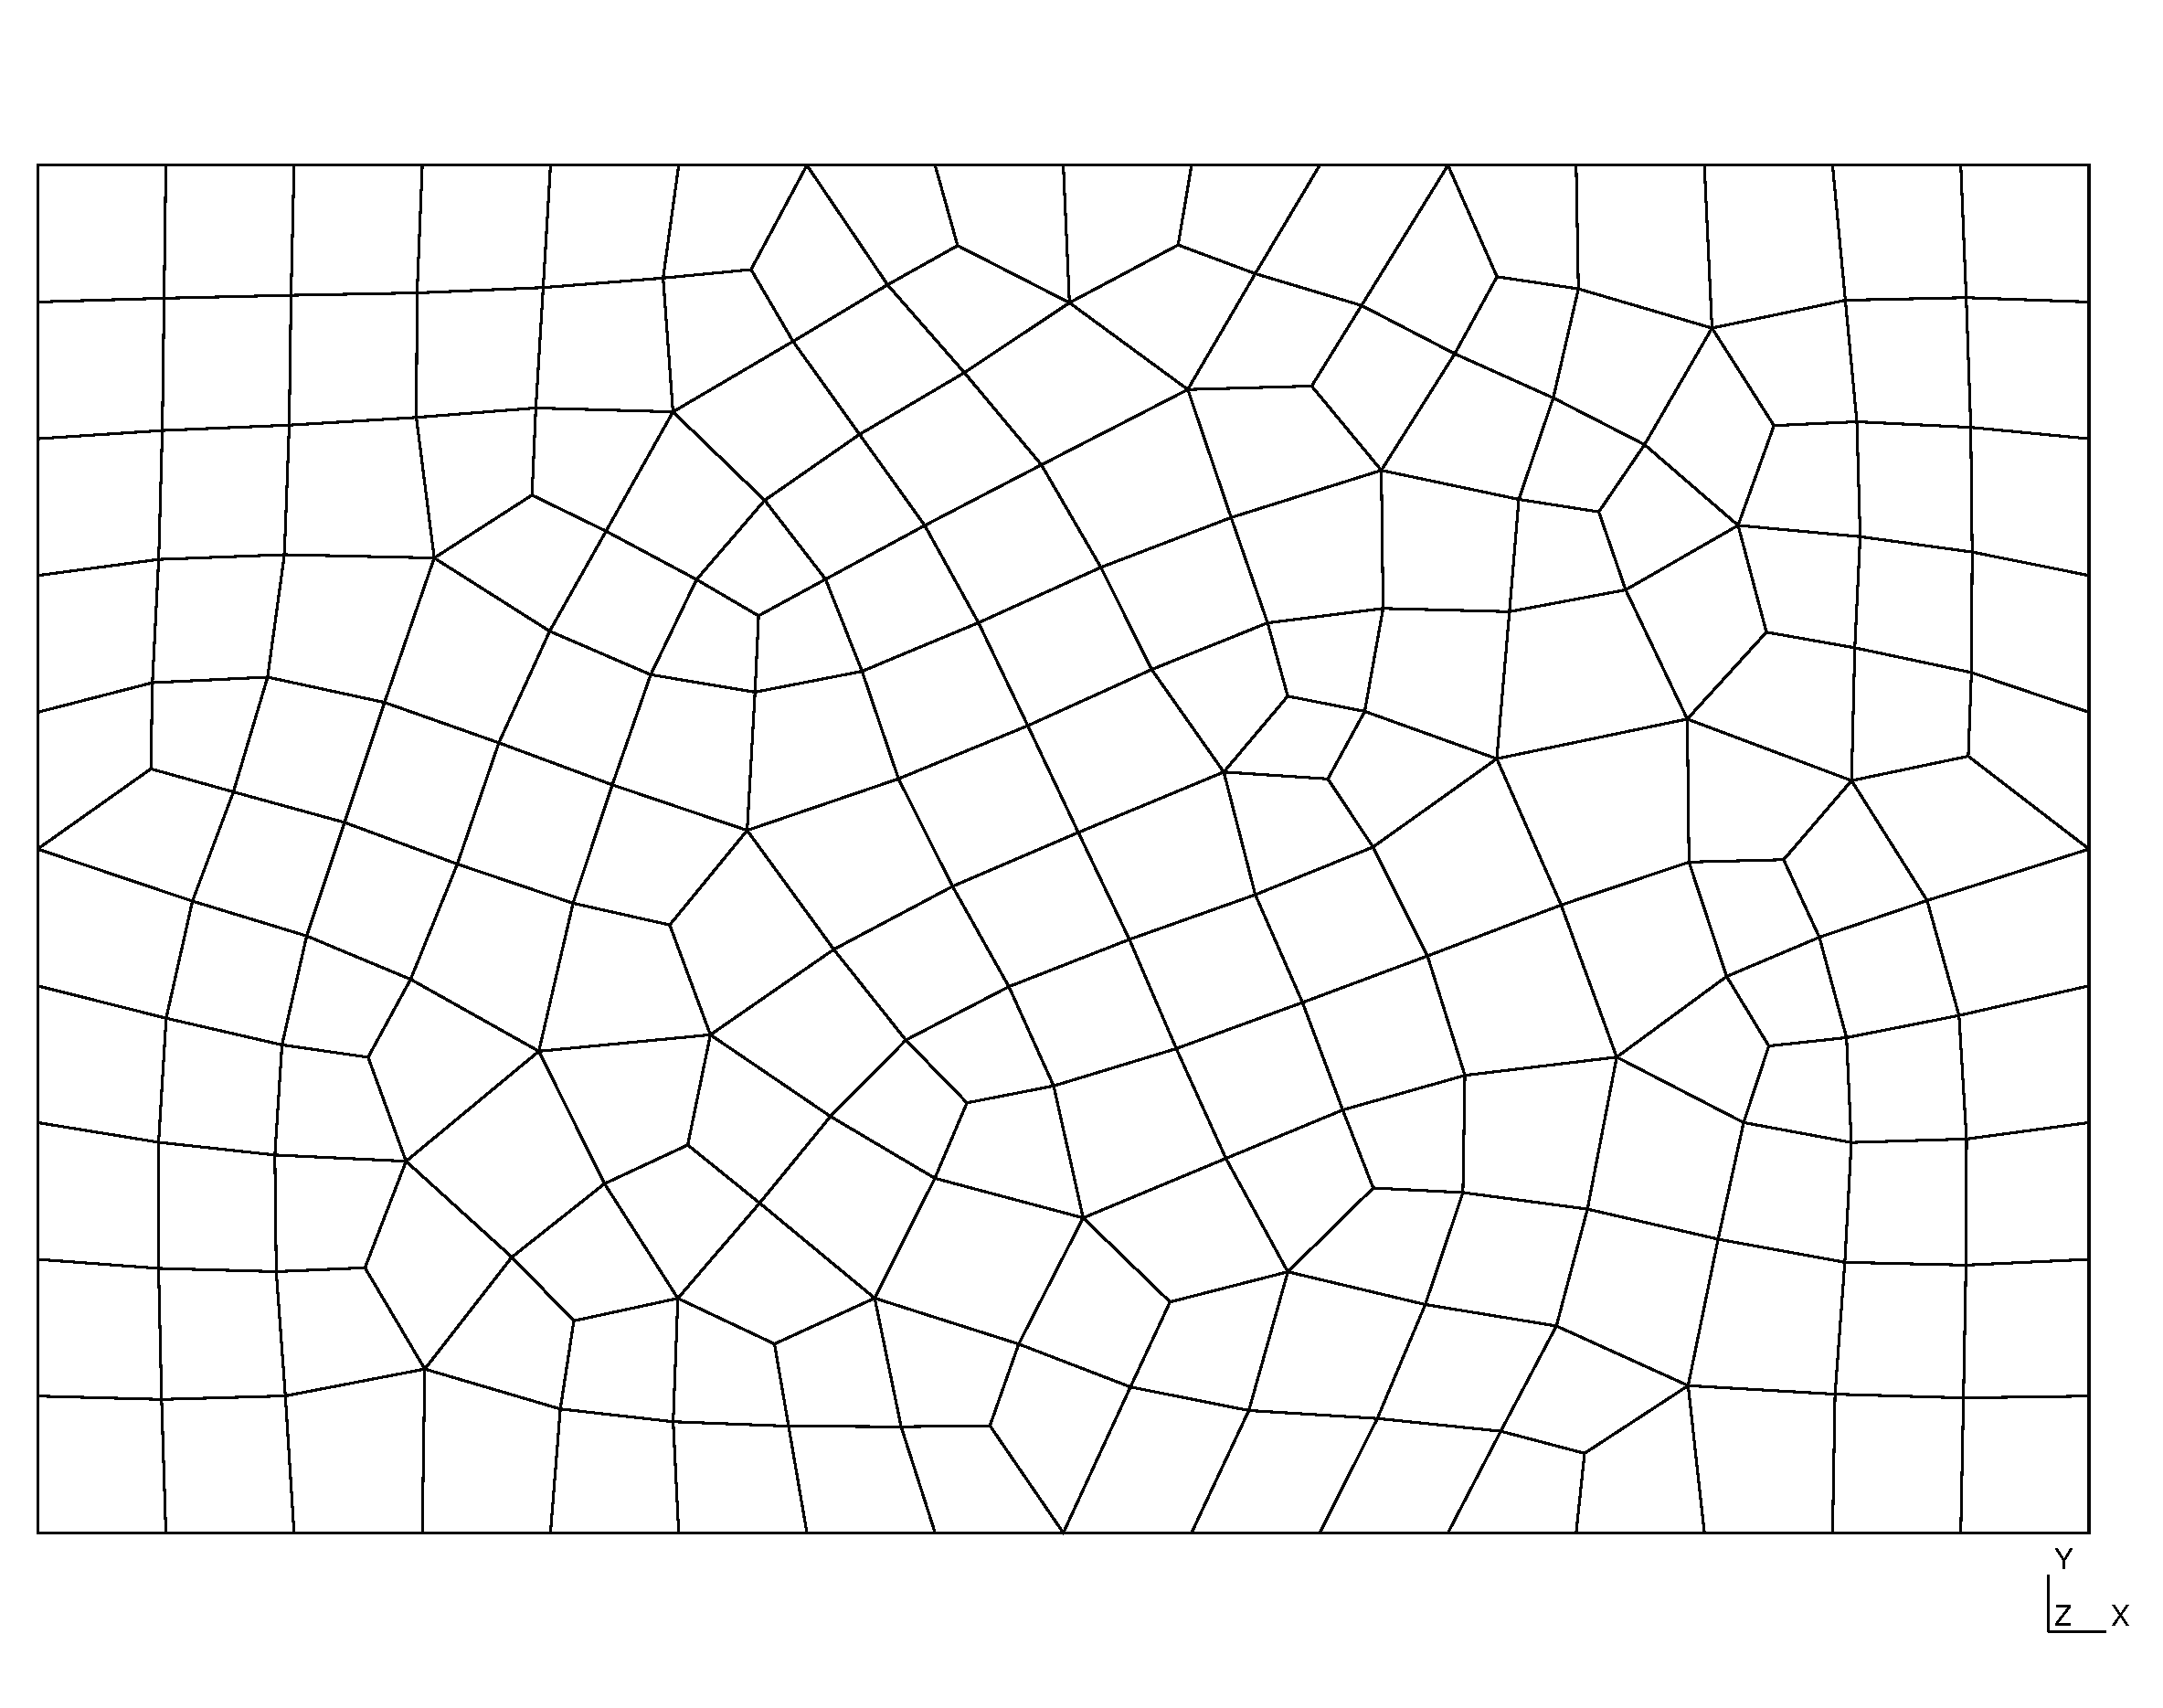
\includegraphics[scale=0.25]{meshquad}
	\caption{One of the quadrangular meshes used}
\end{figure}
\begin{figure}
	\centering
	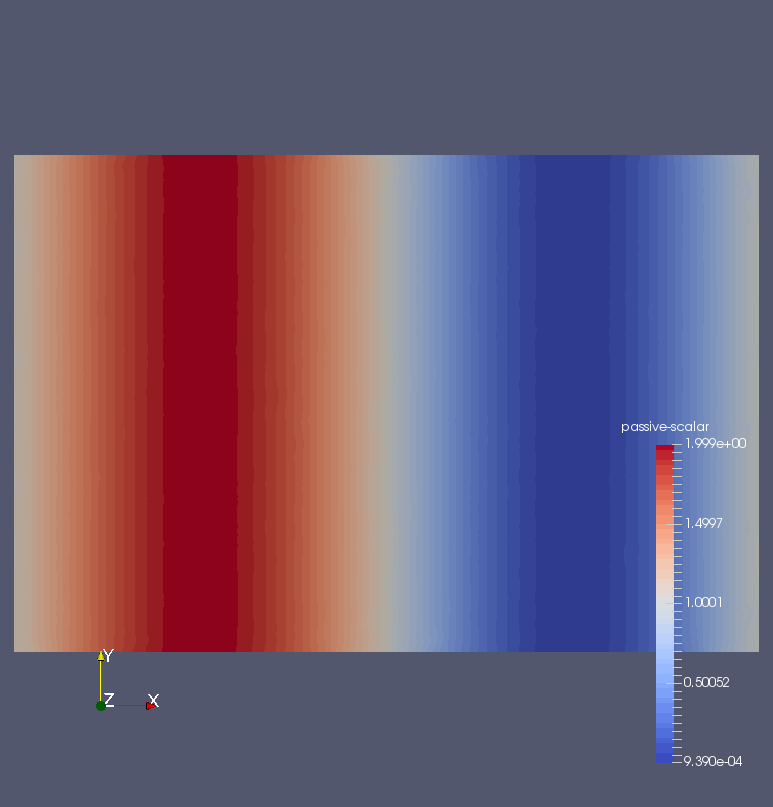
\includegraphics[scale=0.3]{solution-steady-linadv}
	\caption{The solution}
\end{figure}
\begin{figure}
	\centering
	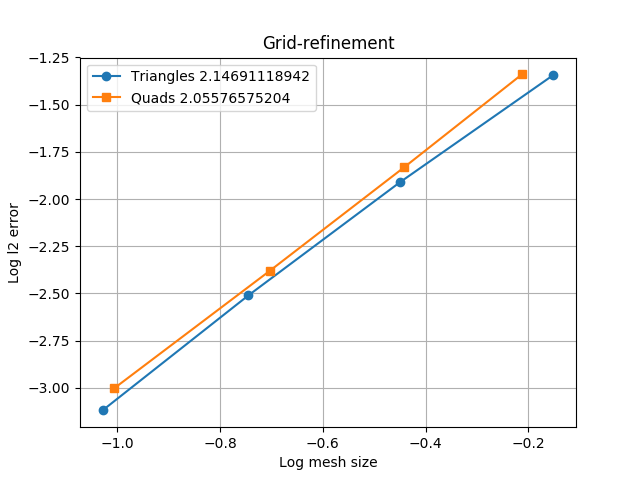
\includegraphics[scale=0.7]{linadv-taylor-p1}
	\caption{Convergence w.r.t. mesh size parameter $h$ for P1}
\end{figure}
\begin{figure}
	\centering
	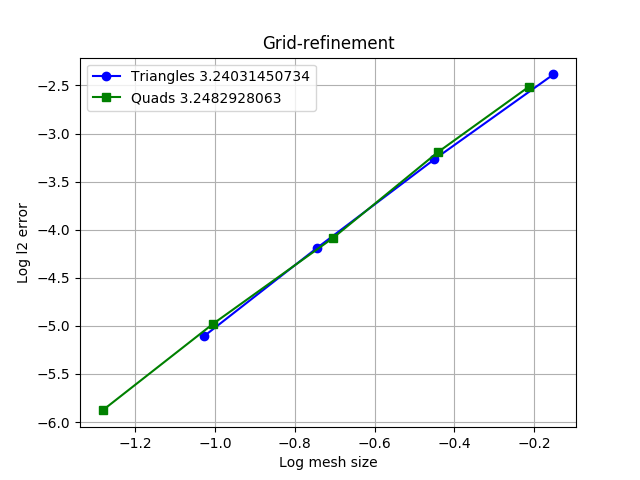
\includegraphics[scale=0.7]{linadv-taylor-p2}
	\caption{Convergence w.r.t. mesh size parameter $h$ for P2}
\end{figure}
\begin{figure}
	\centering
	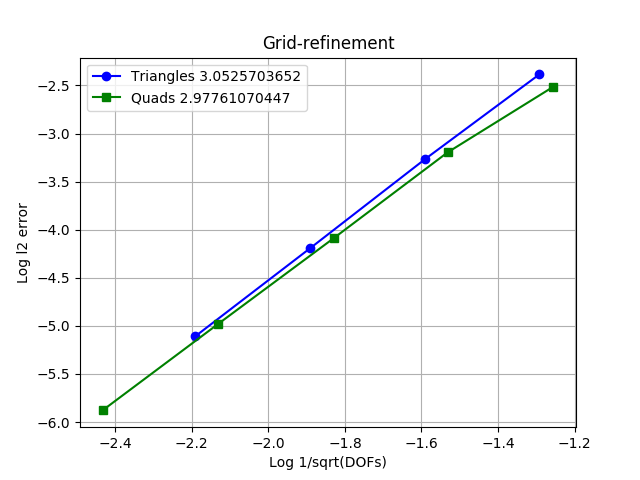
\includegraphics[scale=0.7]{linadv-taylor-p2-dofs}
	\caption{Convergence w.r.t. $\sqrt N_{dof}$ for P2}
\end{figure}

\section{Conclusion}
While a simulation involving reconstruction was not attempted, it has been shown that Taylor basis functions could provide a viable alternative to Lagrange basis functions for simulations of hyperbolic problems. The convenient extension to reconstruction DG to increase the accuracy without an increase in the number of degrees of freedom would be the main motive to use Taylor basis functions.

\bibliography{refs}
\end{document}